\chapter{GFU Fast Fourier Transform}

We begin with the assumption that we are working with a finite viewing window of a sinusoidal rate, $\mathcal{R}$\footnote{here, $\mathcal{R}$ is only the fluctuation from the mean rate, $\mathcal{R} = \frac{r-<r>}{<r>}$, where $r$ is the true rate}:

\begin{equation}
\label{eq:rate}
    \mathcal{R}(f,t,\delta, w) = \Pi \left(\frac{t-\pi  w}{2 \pi  w}\right) \sin (2 \pi  \delta +f t) \; , 
\end{equation}

where $t$ is the time, $f$ is the frequency, $\delta$ is an offset, and our viewing window is encompassed by a unit step function, $\Pi$, with width characterized by $w$. 

We are interested in observing this rate in frequency space, and naturally wish to take a (fast) Fourier Transform (FFT):

\begin{equation}
\label{eq:FFT}
    \mathcal{F}_t[\mathcal{R}(t)](\omega ) = \frac{1}{\sqrt{2 \pi}} \int_{-\infty}^{\infty} \mathcal{R}(t) e^{i \omega t} d t \; .
\end{equation}

We know that in the case of a pure sinusoid, the $\mathcal{F}$ operator should return delta functions corresponding to the frequency of our rate. This is also the case for an infinite viewing window,

\begin{equation}
    \lim_{w\rightarrow \infty} \mathcal{F}_t[\mathcal{R}(t)](\omega ) = i \sqrt{\frac{\pi }{2}} e^{-2 i \pi  \delta } \delta (\omega -f)-i \sqrt{\frac{\pi }{2}} e^{2
   i \pi  \delta } \delta (f+\omega ) \; .
\end{equation}

We are interested in investigating the effect that a limited viewing window has on our FFT. Applying Eq.~\ref{eq:FFT} to our rate function defined in Eq.~\ref{eq:rate}, and taking the magnitude in $\mathbb{C}$, we get 

\begin{multline}
   \mathcal{F}_t[\mathcal{R}(t)](\omega ) =  \Bigg| \frac{1}{4\pi (f^2 - \omega^2)}(\theta (-w)-\theta (w)) (\cos (2 \pi  (\delta +f w-w \omega ))-i \sin (2 \pi  (\delta +f w-w
   \omega ))) \; \times \\ \qquad (2 i (f-\omega ) \sin (\pi  w (f+\omega )) (\cos (4 \pi  \delta +3 \pi  f w-\pi
    w \omega )+i \sin (4 \pi  \delta +3 \pi  f w-\pi  w \omega )) \; +  \\ (-f-\omega ) (i \sin (2 \pi
    f w-2 \pi  w \omega )+\cos (2 \pi  f w-2 \pi  w \omega )-1)) \Bigg| \; ,
\end{multline}

which can be simplified to 

\begin{multline}
    \mathcal{F}_t[\mathcal{R}(t)](\omega ) = \frac{1}{4\pi} \Big| \frac{1}{f^2 - \omega^2} \Big( e^{- 2 \pi i (fw+\delta-w\omega)}\big(-(f+\omega)(-1+e^{2\pi i w(f-\omega)}) + \\ 2i\sin (\pi w(f + \omega)) e^{i(3f\pi w + 4\pi \delta - \pi w \omega)}\big) \Big) \Big|
\end{multline}

A sample time series and the corresponding FFT are displayed in Fig.~\ref{fig:ex_fft}. Here, the effect of the finite viewing window is visible in the separate peaks in the FFT, a consequence often referred to as \textit{spectral leakage}\footnote{For a thorough writeup on spectral leakage, see \url{https://en.wikipedia.org/wiki/Spectral_leakage}.}.
\begin{figure}
    \centering
    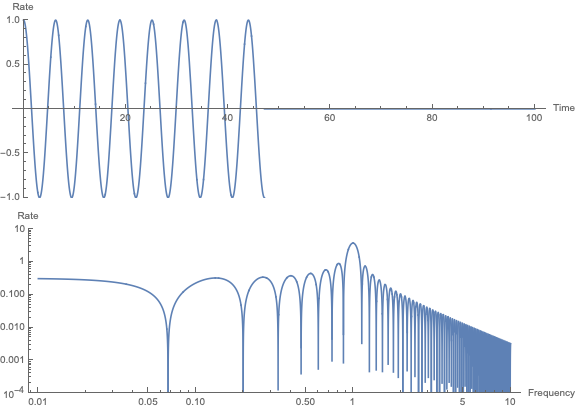
\includegraphics[width=0.90\textwidth]{images/box_fft_sample.png}
    \caption{A sample time series (top) with a pure sine wave and finite viewing period (7.5 cycles) with corresponding FFT (bottom)}
    \label{fig:ex_fft}
\end{figure}
In the gamma-ray followup (GFU) dataset, it has been noted in the past that the effects of seasonal variations are evident, and manifest in an overall $\mathcal{O}$(10\%) fluctuation in the background rate. 

For short timescale analyses, an accurate prediction of the background rate is of utmost importance in quantifying the significance of a possible signal. As a result of seasonal variations, calculating the rate from the entire livetime of the dataset leads to systematic over- and under-estimations of the rate, whereas parameterizing the background rate from data around the time of a transient event is limited by statistical fluctuations of the rate. In order to see if we can model the rate as a sinusoid, we take an FFT of the rate data, and try to make sure that any features can be explained by what is expected from an FFT of a windowed sinusoid.
\begin{figure}
    \centering
    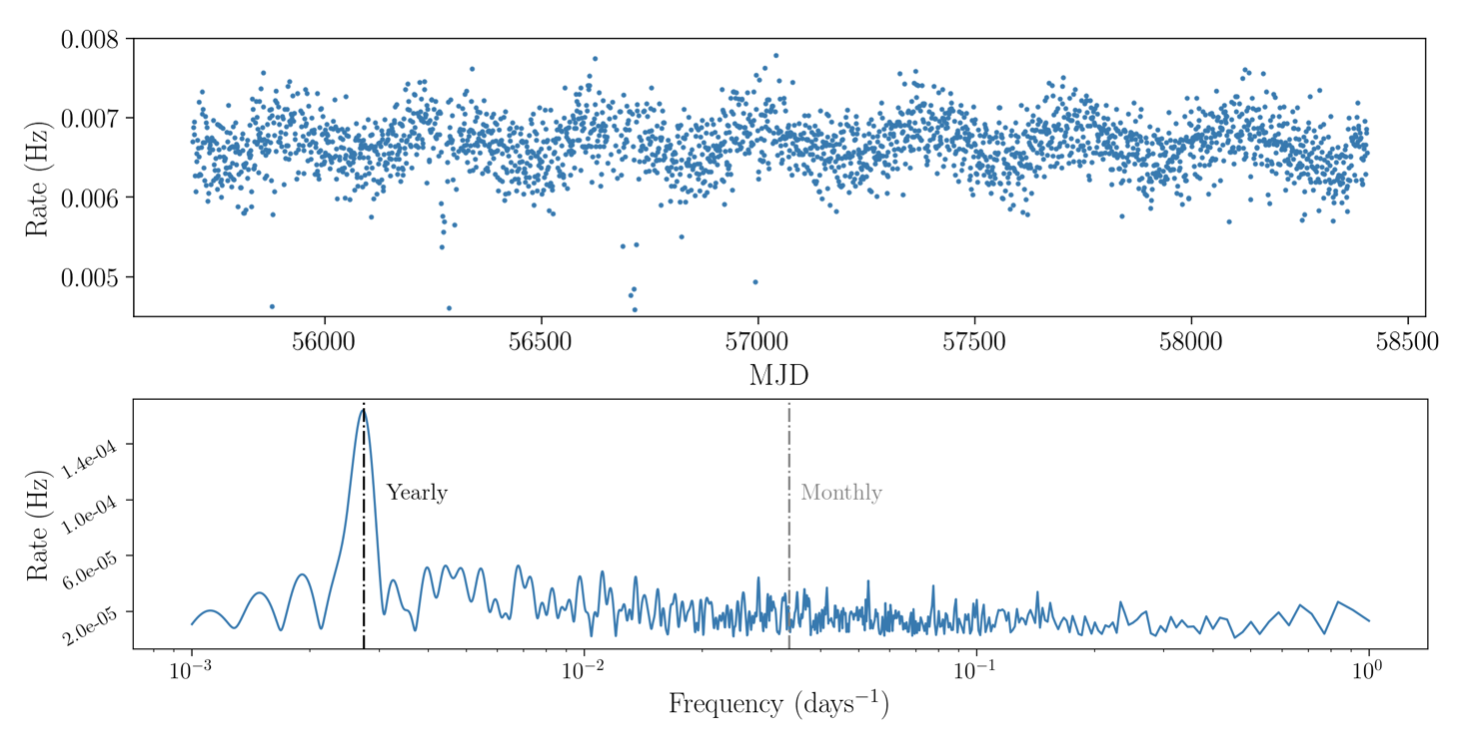
\includegraphics[width=0.9\textwidth]{images/gfu_sample_sidebyside.png}
    \caption{GFU time series (top) and FFT (bottom) for 7.5 years of data}
    \label{fig:gfu_7_year_fft}
\end{figure}

Fig.~\ref{fig:gfu_7_year_fft} shows the rate time series and corresponding FFT for the 7.5 years of available data from GFU. Here, as the data is sampled unevenly, we use the Lomb-Scargle periodogram\footnote{For details on the algorithm, see \url{https://arxiv.org/abs/1703.09824}.} algorithm to transform these data into frequency space. There is clear structure to the left of the annual peak. To investigate if these are the expected peaks, we extremize numerically. And find that there should be peaks at frequencies of $\{0.41,0.54,0.67,0.8\}\times f_0$, where $f_0$ is the peak frequency in the plots in the figures above. The numerical derivative has some odd structure, and is displayed below

\begin{figure}
    \centering
    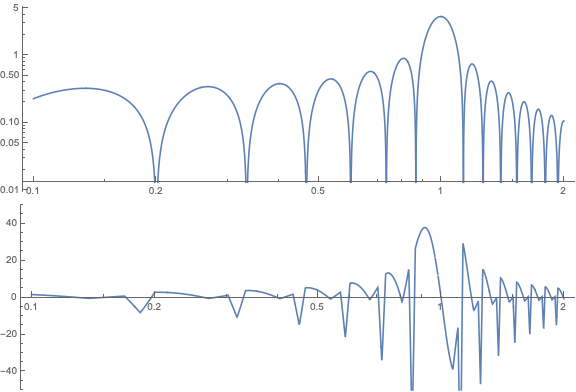
\includegraphics[width=0.75\textwidth]{images/GFU_fft_with_derivative.png}
    \caption{FFT (top) and numerical derivative of FFT (bottom)}
    \label{fig:fft_derivative}
\end{figure}

Placing lines at the corresponding frequencies in the GFU FFT results in Fig.~\ref{fig:gfu_with_harmonics}

\begin{figure}
    \centering
    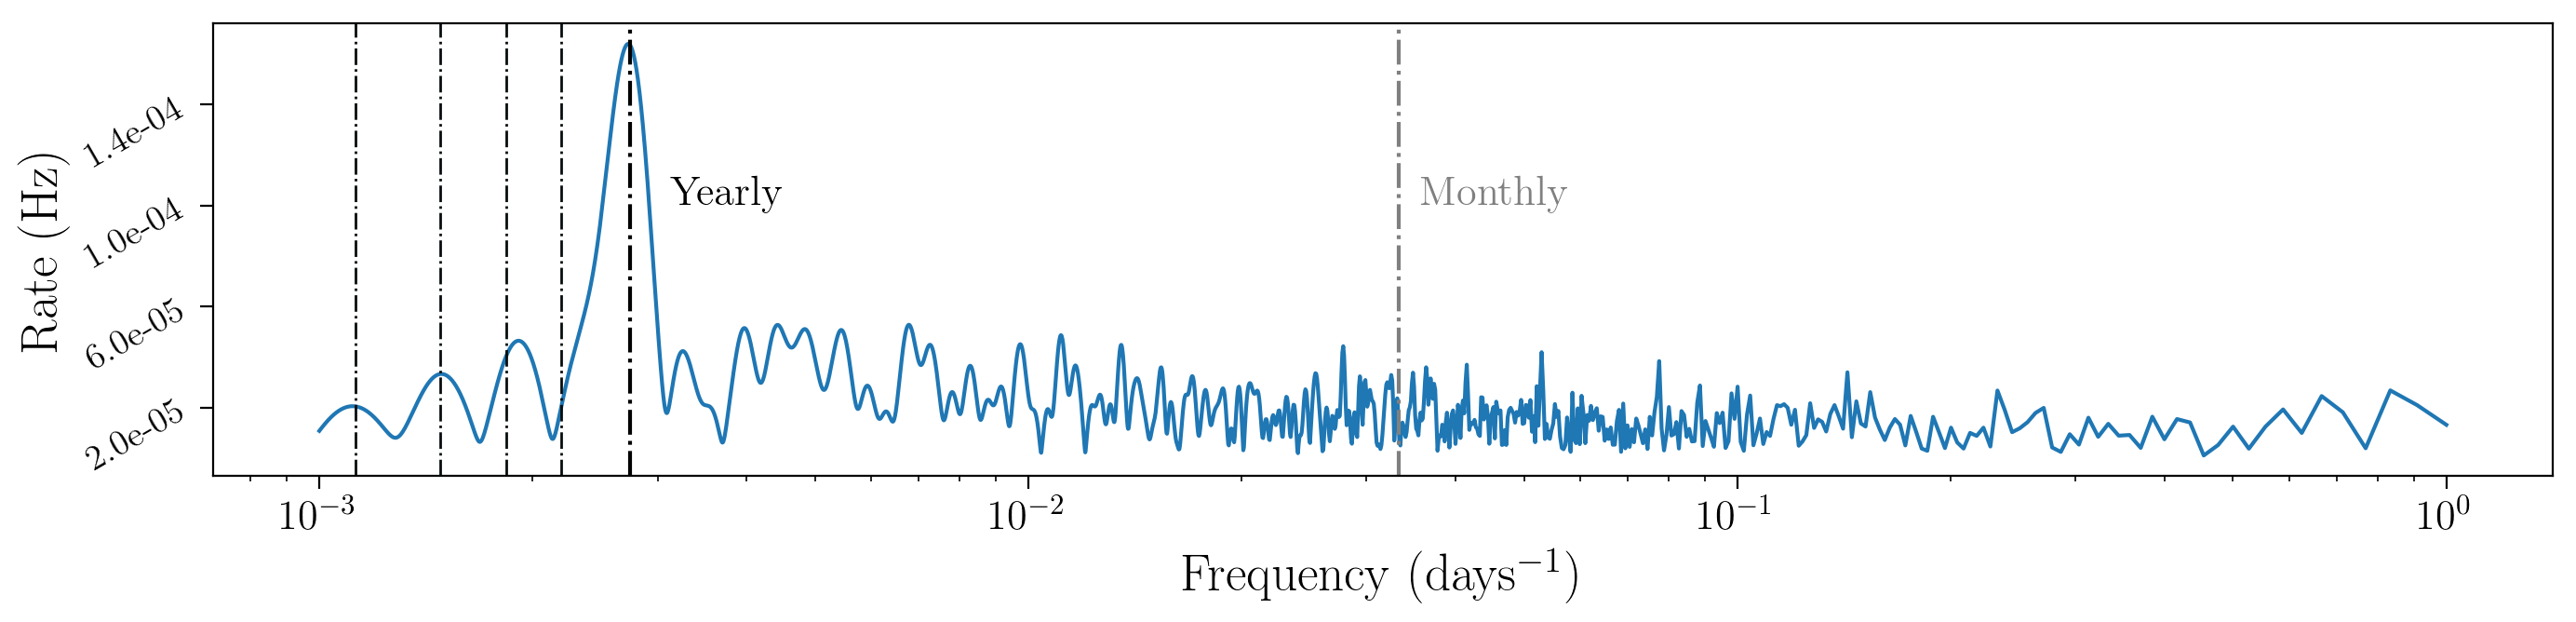
\includegraphics[width=0.95\textwidth]{images/gfu_with_correct_harmonics.png}
    \caption{GFU FFT with additional lines at the locations of the extremal frequencies extracted from Fig.~\ref{fig:fft_derivative}}.
    \label{fig:gfu_with_harmonics}
\end{figure}